\chapter{Identification of Non-photonic Electrons}

We discuss the procedure for identifying electrons in events at STAR and how we remove photonic background. We show the event and track selection criteria and then lastly we will analyze the efficiency for identifying background photonic electrons. The identification of non-photonic electrons (NPE) and efficiency thereof will be critical factors when we construct the NPE-hadron correlations in later chapters.

\section{Outline of the NPE Identification}

This chapter will lay out the general methods for event selection, track selection, electron identification, and the removal of photonic electron background for both Au+Au and p+p collisions.

We start by identifying the dataset and the trigger collections we will use for the analysis. We look at the events and check that the quality of the event is good and that there could be candidate tracks for NPE in the event. We then reconstruct all tracks in the TPC and apply track quality cuts. To identify electrons we rely on the energy loss ($dE/dx$) measured in the TPC and on the hits in the EMC towers and shower max detector. 

The background from photonic electrons will be removed by searching for the opposite signed partner electron. If the primary track is from Dalitz decays or photon conversion in the detector, the partner and primary track should have a low invariant mass. We will also investigate, through simulations, the efficiency for determining the background from photonic electrons.

In the end we will have a sample of electrons which we can use as triggers for measuring NPE-hadron correlations. 

\section{Dataset and Event Selection}

\subsection{Data and Triggers}

In 2011 RHIC collided gold nuclei at $\sqrt{s_{NN}} = 200$ GeV and delivered 9.79 $nb^{-1}$ integrated luminosity similar to what was delivered during the previous year's run (Figure~\ref{fig:Luma}). The STAR detector recorded about 1.1 billion events across all triggers with TPC and BEMC information. In 2012 polarized proton collisions were run in RHIC (the polarization of the beams is not relevant to this analysis) at the same 200 GeV beam energy. RHIC delivered 74.0 $pb^{-1}$ (Figure~\ref{fig:Lumb}) which resulted in 1.7 billion triggered events in STAR. Heavy flavor events are rare and detector efficiencies can be low meaning the NPE analysisis typically constrained by statistics, necessitating large data sets. The Silicon Vertex Tracker (SVT) was removed from STAR resulting in less material near the beam line which cuts down on background from conversions in the detector. This combination of low material and high statisics make runs 11 and 12 (prior to run 14) the best datasets available for the analysis of non-photonic electrons.

\begin{figure}[htbp]
    \begin{subfigure}{0.5\textwidth}
        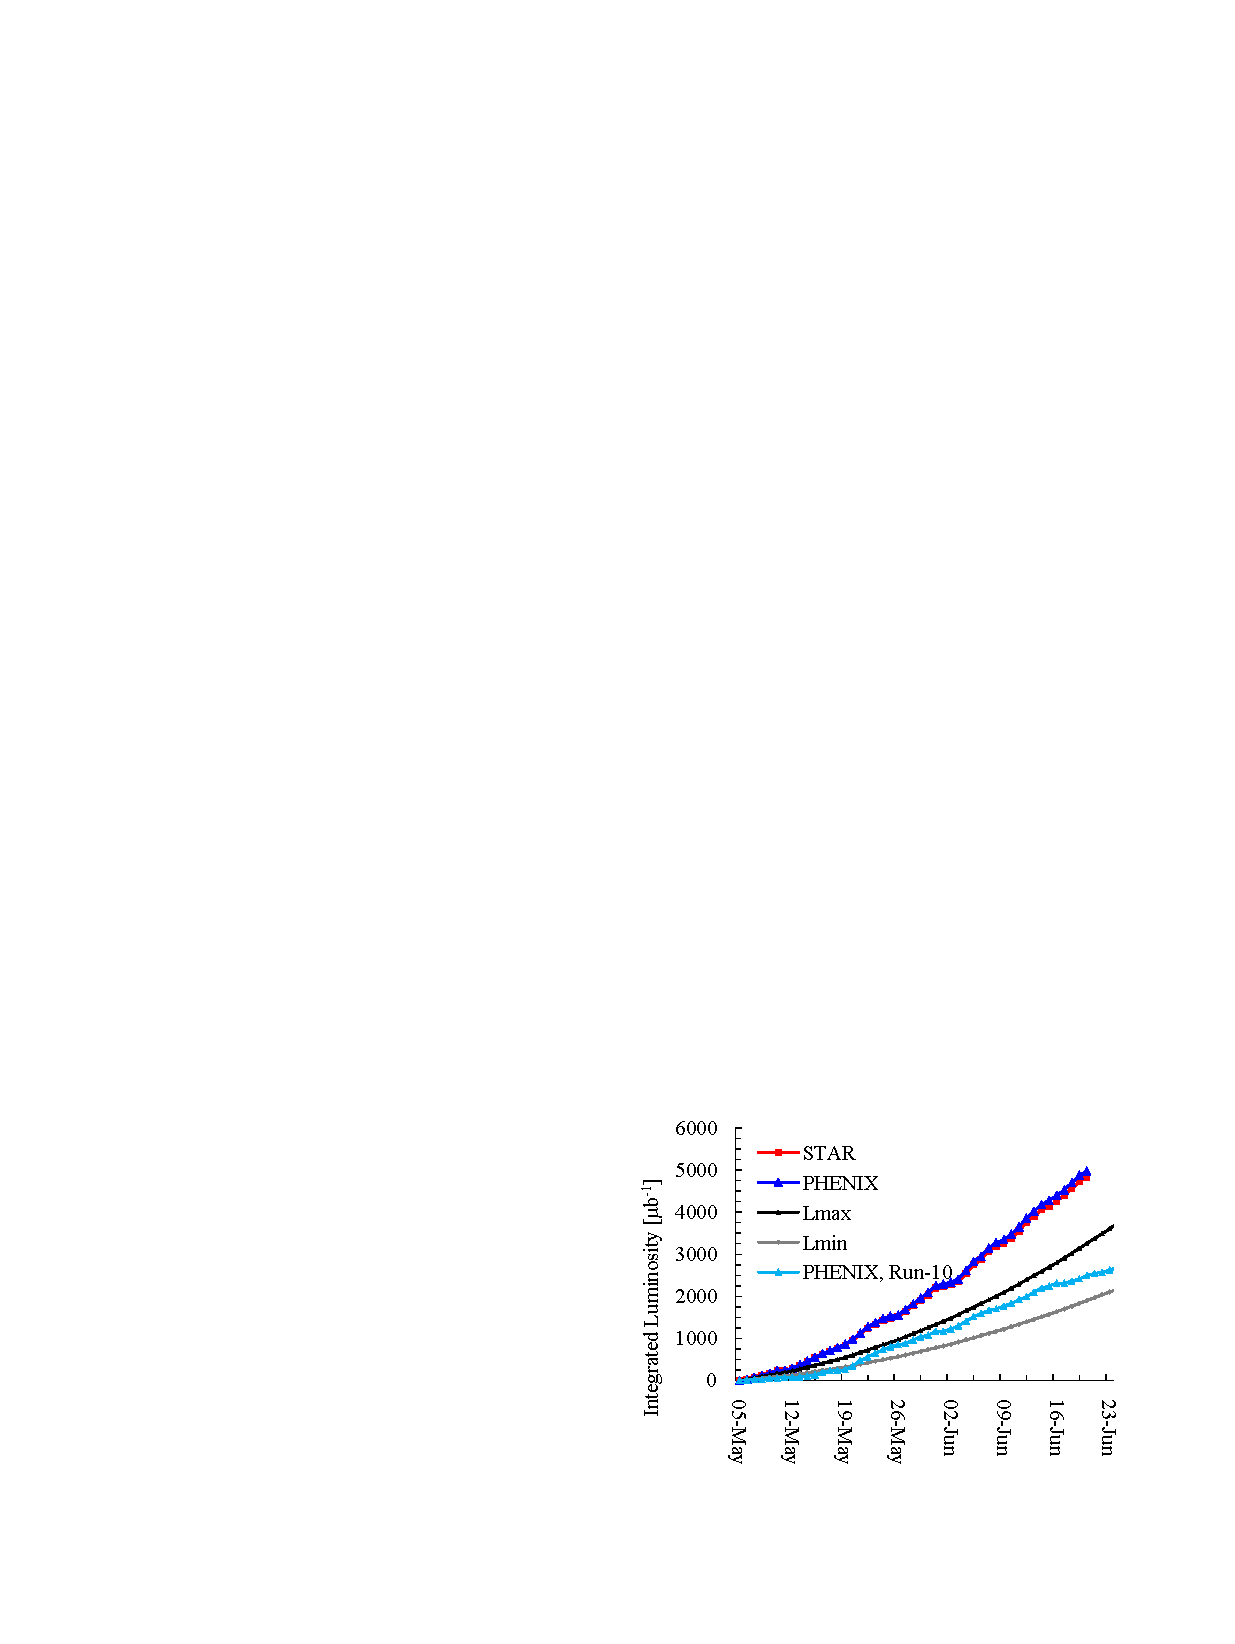
\includegraphics[width=\textwidth]{Plots/NPE/Run11_Lum.pdf}
        \caption{Run 11 Au+Au Integrated Luminosity}
        \label{fig:Luma}
    \end{subfigure}
    \begin{subfigure}{0.5\textwidth}
        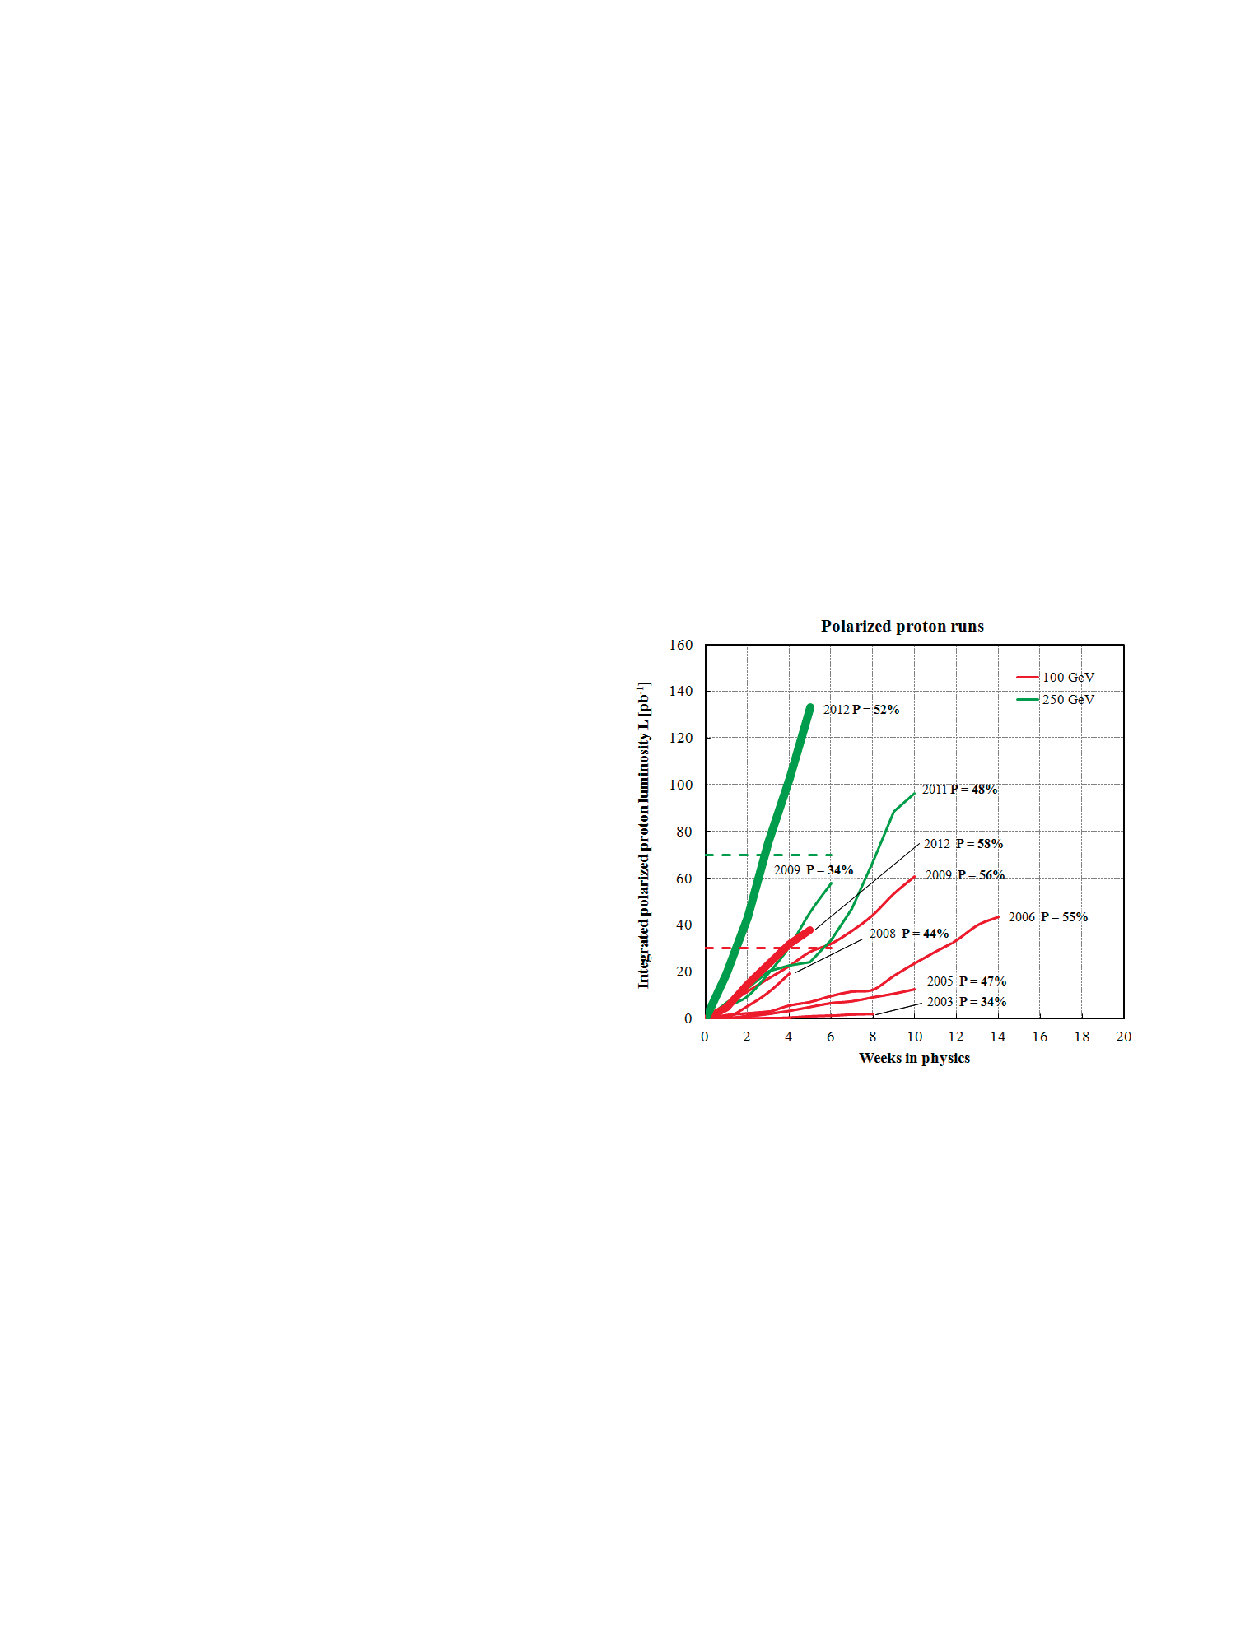
\includegraphics[width=\textwidth]{Plots/NPE/Run12_Lum.pdf}
        \caption{Run 12 p+p Integrated Luminosity}
        \label{fig:Lumb}
    \end{subfigure}
\caption[RHIC Integrated Luminosities in Run11 and Run12]{Integrated luminosities for run 11 and run 12 in RHIC. Left plot shows Au+Au delivered to STAR and PHENIX as well as run 10 in PHENIX for comparison. Right plot shows all p+p runs, run 12 is shown with thick lines.}
\label{fig:RunLum}
\end{figure}

The STAR data acquisition system handles several different triggers the most commonly used is the minimum bias trigger (minbias) which fires based on the coincidence of the STAR vertex position detector(VPD) and Zero Degree Calorimeters (ZDC) these events are prescaled so that only a fixed fraction of triggers are accepted so that the DAQ's data taking rate is not exceeded. STAR can also trigger on hits in the barrel EMC, these are the high tower (HT) triggers. A high tower trigger requires that a hit in a BEMC tower exceeds an ADC threshold determined such that the transverse energy in that tower is high. In run 11 we use the HT triggers NPE11, NPE15, NPE18, and NPE25 which are in increasing order of $E_{T}$. The NPE11 and NPE15 triggers are also prescaled. In p+p we use the BHT0, BHT1, BHT2, and BHT3 triggers, of these only BHT0 is prescaled.

Due to the large dataset sizes it is in our best interest to cut down on the data we need whenever possible. We do this first when we read the data to make BEMC points to match to tracks. Here we look through the tracks in the event and search for electron candidates based on the TPC information only. We throw out events without viable electron candidates. Since these cuts are looser than the electron cuts we will apply later we don't remove events we might actually want and we retain the ability to tighten the cuts later if we need to. After limiting ourselves to high tower triggers and keeping only events with electron candidates we are left with approximately 23 million events in Au+Au and 1.1 million events in p+p.

\subsection{Event Level Cuts}

At the event level we cut on events with vertex too far out of the center of the detector. We use the tracks in the TPC to reconstruct the vertex, we can also measure the vertex with the Vertex Position Detector (VPD). By convention we have the $x$ and $y$ axes as transverse to the beam line. The $z$ axis then runs along the beam. We require that the vertex be no more than 2 cm from the center of the beam pipe in the radial direction, i.e. $\sqrt{(V_x^{TPC})^2 + (V_y^{TPC})^2} \leq$ 2 cm. We also cut on the TPC vertex in the $z$ direction, choosing events with $|V_z^{TPC}| \leq$ 30 cm in Au+Au collisions and $|V_z^{TPC}| \leq$ 40 cm in p+p. Additionally we want to have good agreement between the vertices as measured by the TPC and VPD. We require that the difference between the measured $V_z$ satisfies $|V_z^{TPC} - V_z^{VPD} \leq|$ 4 cm in Au+Au. Figure~\ref{fig:Vertexz} shows the distribution of $V_z^{TPC}$ and the difference in TPC and VPD $V_z$ in Au+Au collisions. In p+p because of lower multiplicity and a wider vertex distribution the measured vertex from VPD is not reliable and thus the cut on the difference of $V_z$ is not used.

\begin{figure}[htbp]
    \begin{subfigure}{0.5\textwidth}
        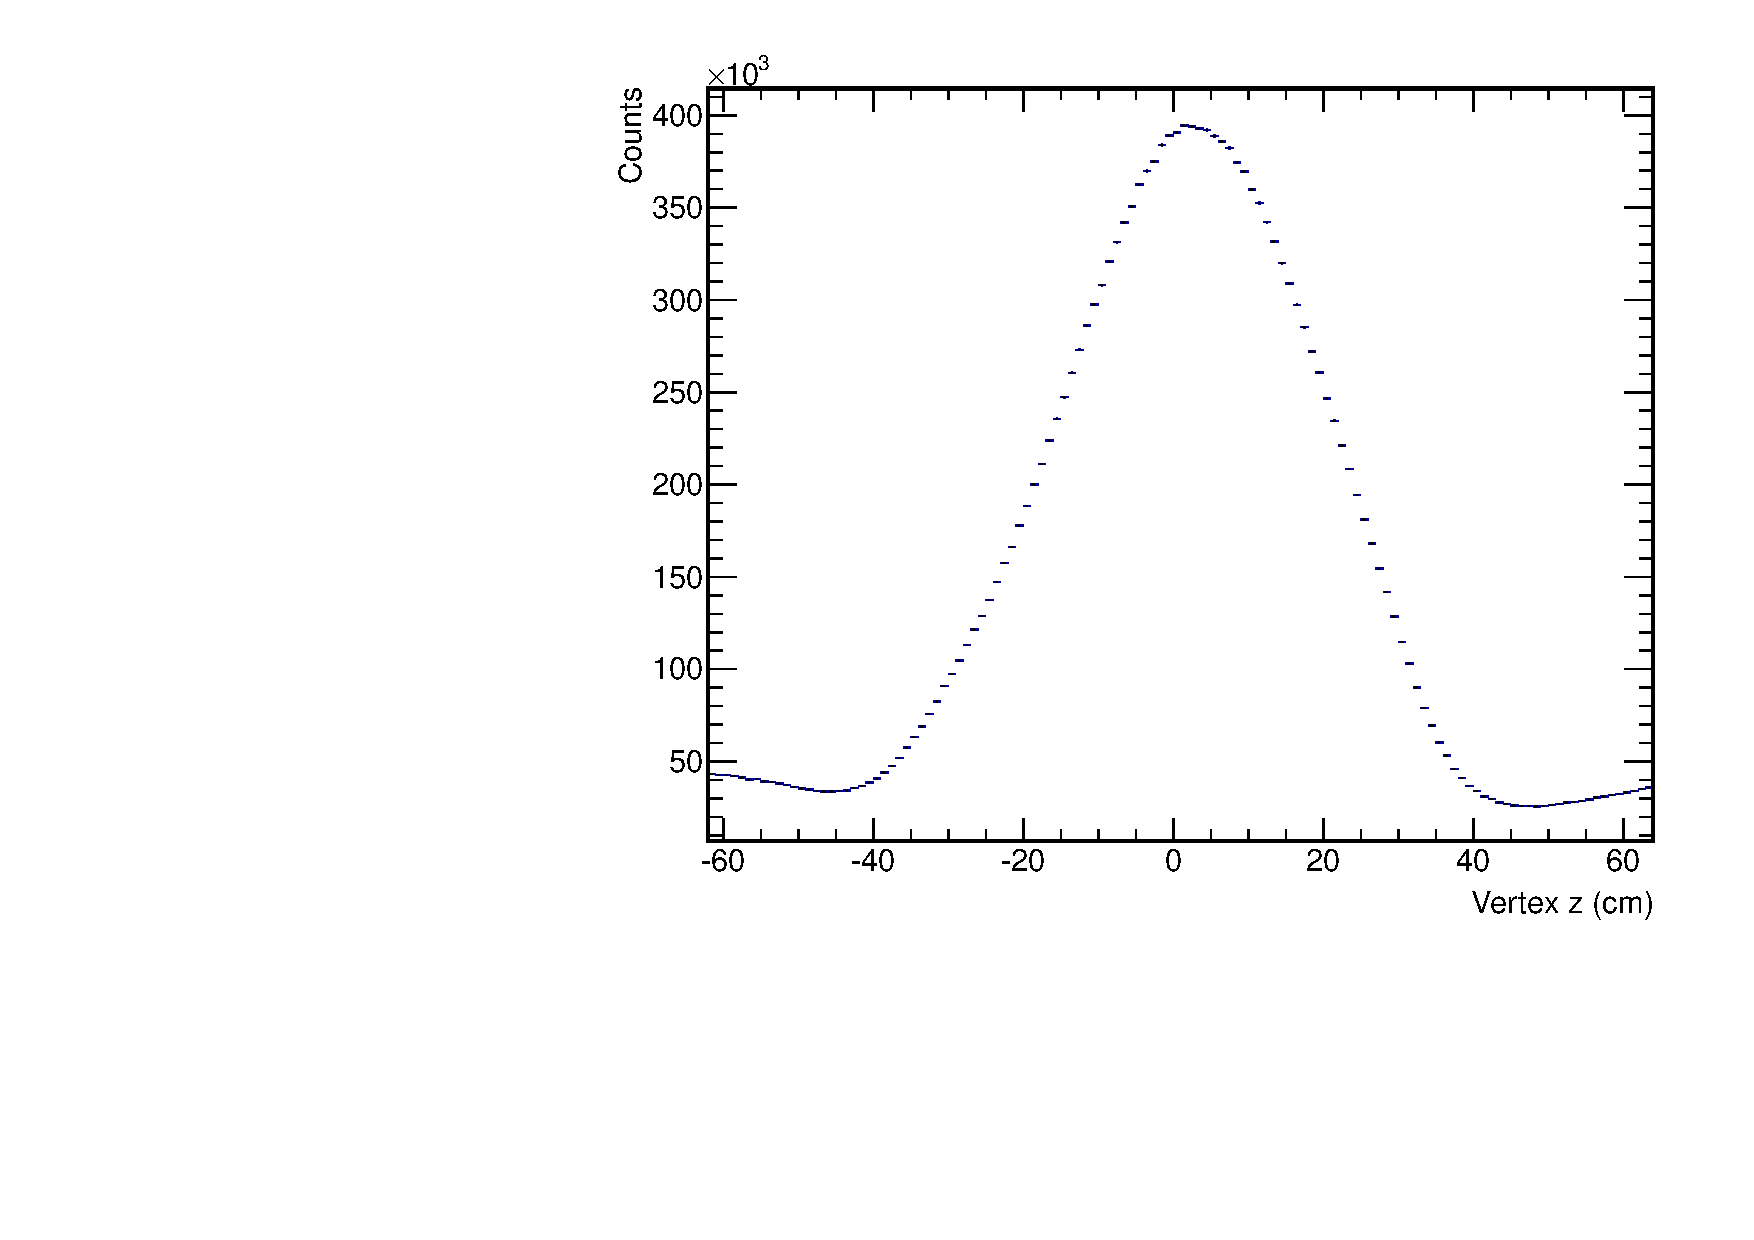
\includegraphics[width=\textwidth]{Plots/NPE/VzAuAu.pdf}
        \caption{$V_{z}^{TPC}$}
        \label{fig:VzAuAu}
    \end{subfigure}
    \begin{subfigure}{0.5\textwidth}
        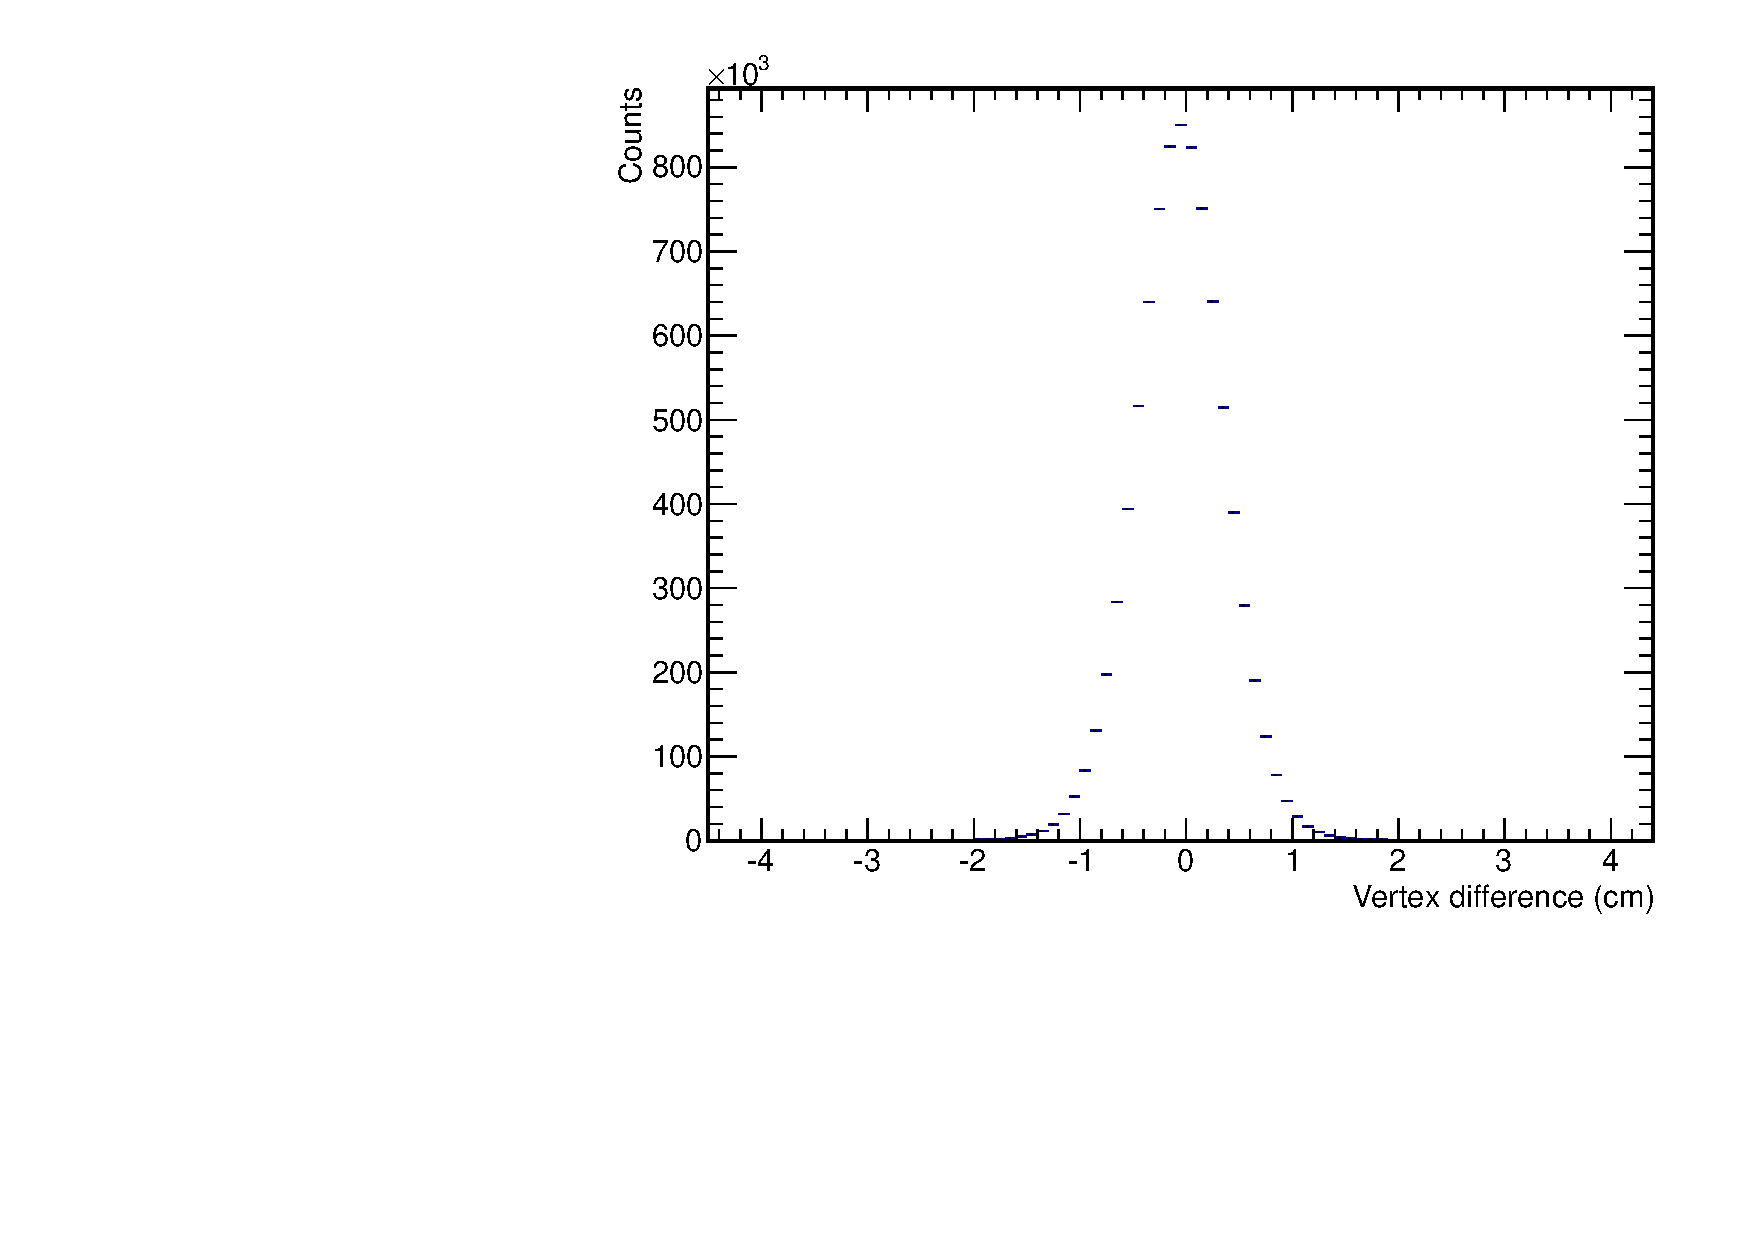
\includegraphics[width=\textwidth]{Plots/NPE/VzDiff.pdf}
        \caption{$V_z^{TPC} - V_z^{VPD}$}
        \label{fig:VertexDiff}
    \end{subfigure}
\caption[TPC $V_z$ and TPC VPD Difference]{Vertex z distribution in run 11 Au+Au. Left plot shows the distribution of the z vertex (cut at $\pm$30 cm), right plot shows the difference between TPC and VPD $V_z$ (cut at $\pm$4 cm).}
\label{fig:Vertexz}
\end{figure}

At the event level we also determine the centrality using the STAR \texttt{StRefMultCorr} class which calculates the centrality bin based on the reference multiplicity (refmult), vertex z, run number, and ZDC coincidence rate. Figure~\ref{fig:EventCent} shows the event by event distribution of refmult as well as the number of events from each centrality bin used in the NPE analysis.
 
\begin{figure}[htbp]
    \begin{subfigure}{0.5\textwidth}
        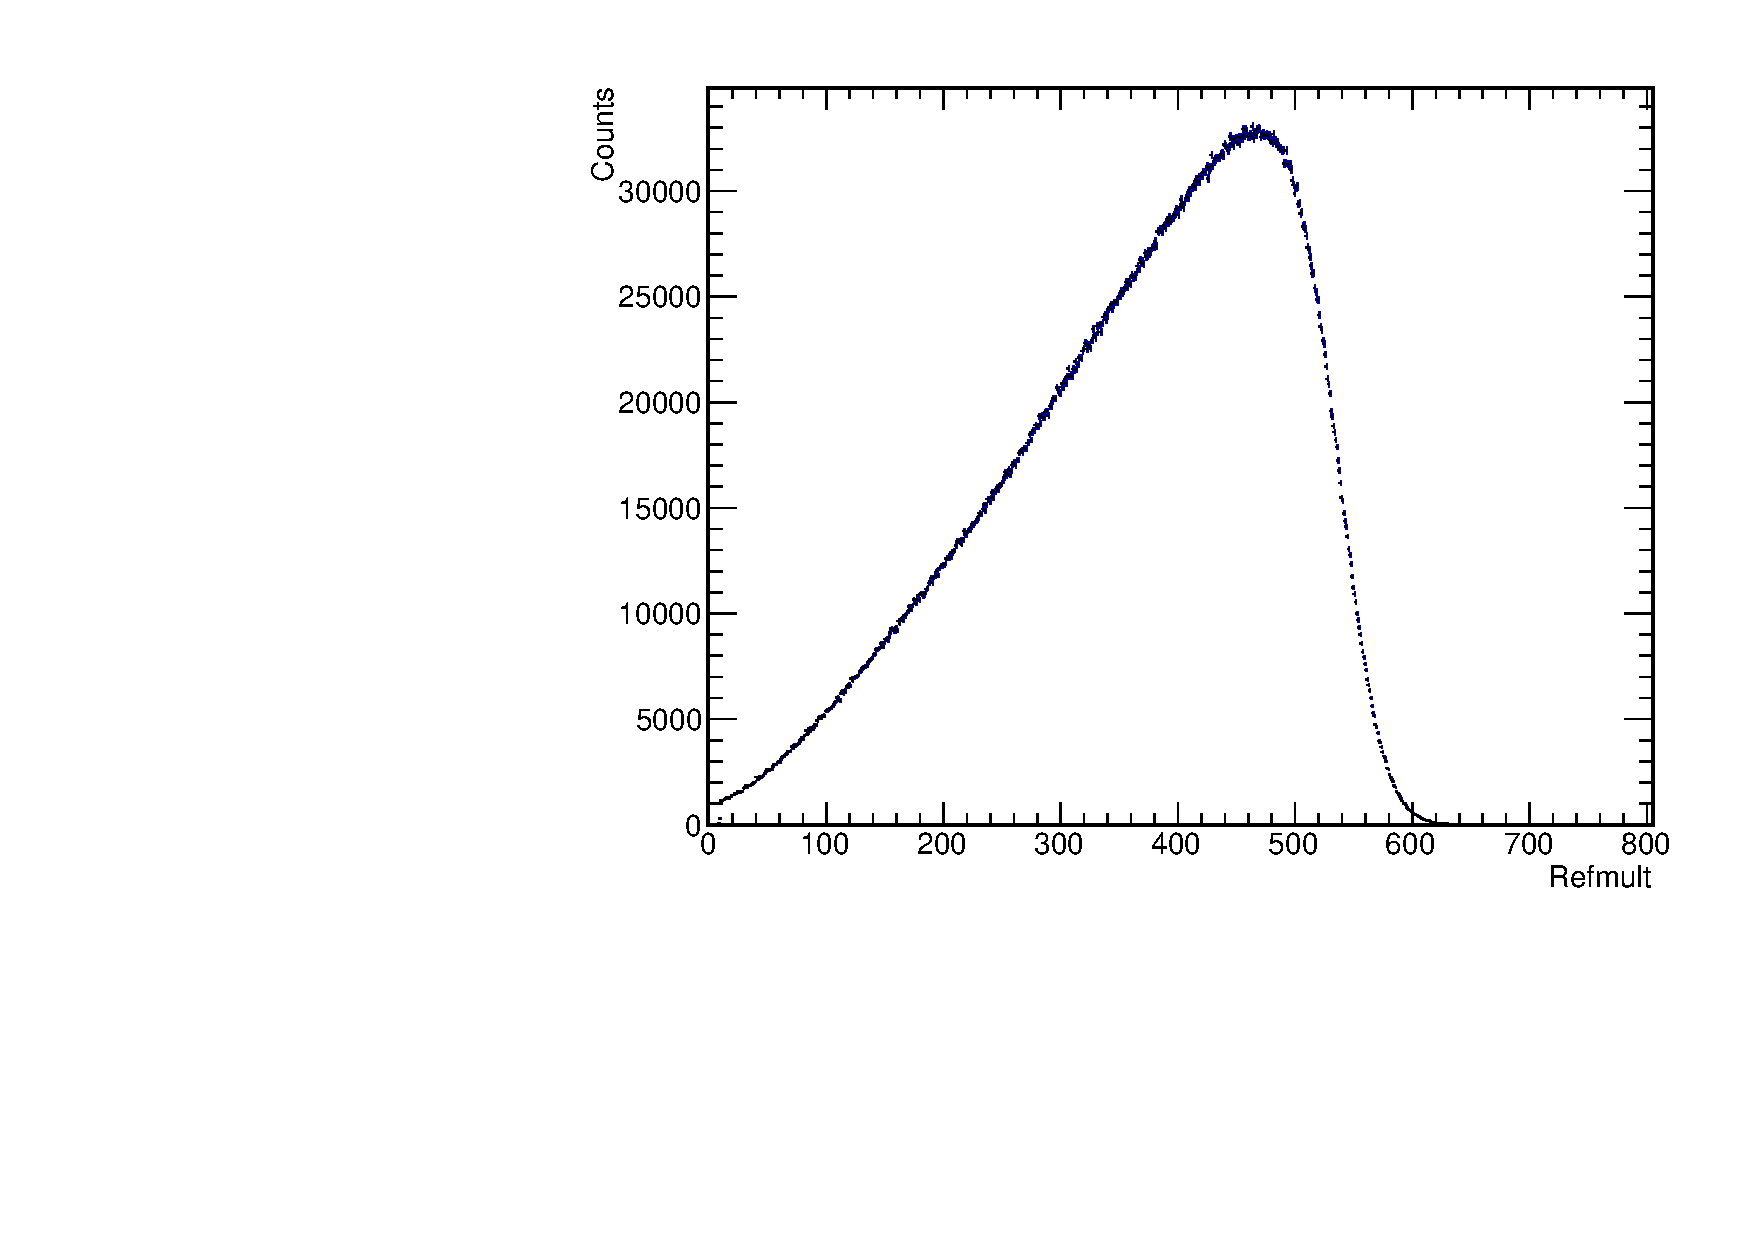
\includegraphics[width=\textwidth]{Plots/NPE/RefmultNPE18.pdf}
        \caption{Reference Multiplicity}
        \label{fig:refmult}
    \end{subfigure}
    \begin{subfigure}{0.5\textwidth}
        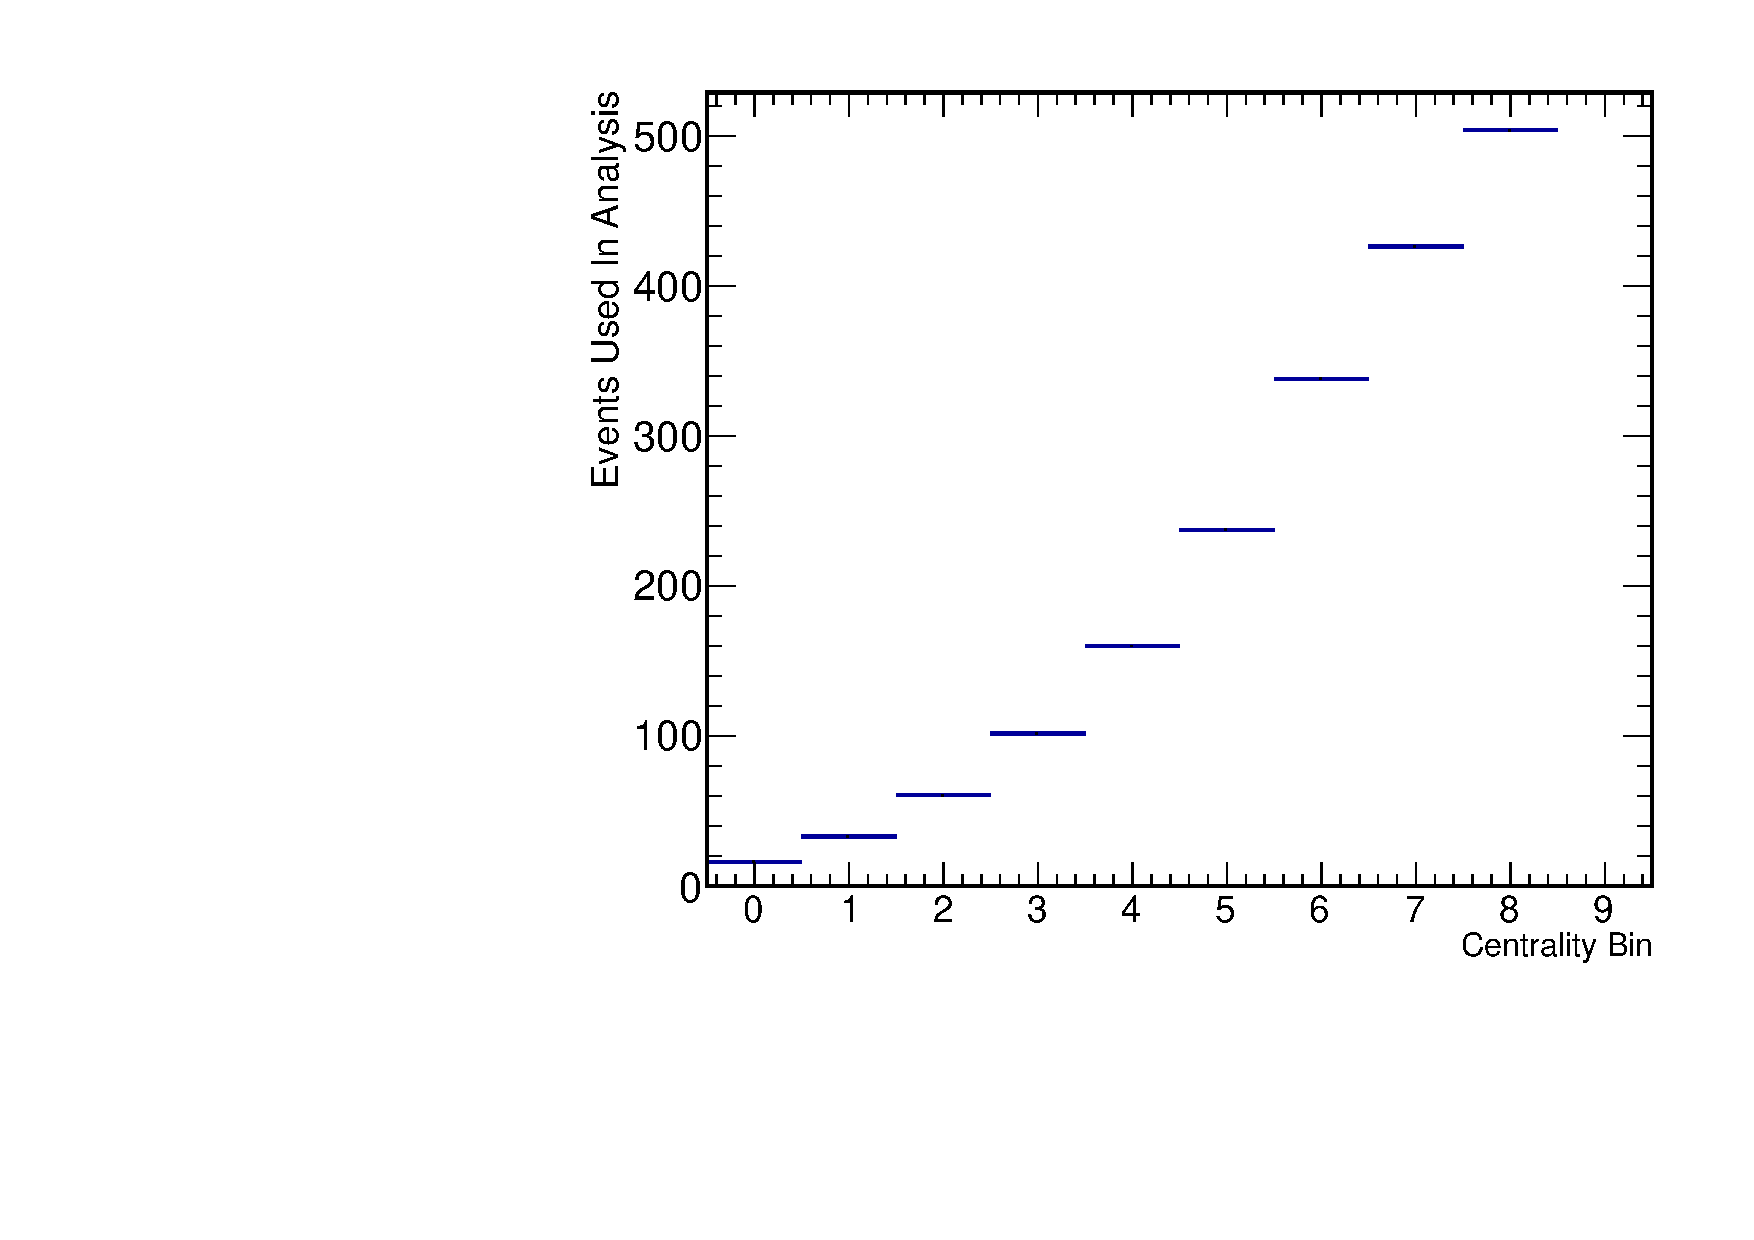
\includegraphics[width=\textwidth]{Plots/NPE/Centrality_dist.pdf}
        \caption{Centrality bins}
        \label{fig:centdist}
    \end{subfigure}
\caption[Refmult and Centrality Distributions]{Reference multiplicity and centrality bin distributions for HT trigger events in Au+Au.}
\label{fig:EventCent}
\end{figure}

\section{Track Reconstruction and TPC Cuts}

The TPC is the primary tracking and particle identification system in STAR. Charged particles traverse the TPC chamber which ionizes the gas inside. Due to the nearly uniform electric field in the TPC these ions drift to the ends of the TPC where the currents are read out by the TPC padrows. The magnetic field in the TPC causes charged particle trajectories to be helical making charge sign distinction possible. We can also use the TPC for particle identification by measuring the ionization energy loss in the detector. 

In the TPC we consider two types of tracks. The global tracks are those tracks from the fit to hits inside the TPC. If a global track has a distance of closest approach (DCA) to the primary vertex less than 3 cm then the primary vertex is added to the track hits and the track is refit. The resulting track is a primary track, which should represent particles coming directly from the collision.

We impose track quality cuts to make sure the track fits are good and that we get a good measurement of $dE/dx$. For primary tracks we require the number of TPC hits used in the track fit is between 20 and 50. For global tracks we only require that the number of hits is above 15. For all tracks we also cut on the ratio of hits fit to the maximum number possible keeping it between .52 and 1.05.

In run 11 and run 12 we have no tracking information near the beam pipe, the Silicon Vertex Tracker was removed before the runs and the new Heavy Flavor Tracker had not been installed. Due to the relatively short decay length (~100 $\mu$m) of $D$ and $B$ mesons this means that the decay vertex of these particles can not be distinguished from the primary vertex. For electron candidates we require primary tracks with DCA of less than 2 cm. The corresponding global track for that electron must also be less than 3 cm. 

The energy loss ($dE/dx$) in the TPC is modeled by the Bichsel function which also accounts for the spread in values for different particle species. We will be looking at the deviation of the energy loss compared to the Bichsel function value for electrons. This quantity is called $n\sigma_e$ and is defined as:

\begin{equation}\label{eq:nsigmae}
n\sigma_e = \frac{\log{\frac{dE/dx}{B_e}}}{\sigma_e}
\end{equation}

where $B_e$ is the Bichsel function value and $n\sigma_e$ is the deviation from the mean Bichsel function value for electrons. Analagous values are defined for protons, kaons, and pions but we will only concern ourselves with $n\sigma_e$. We will go over the specific $n\sigma_e$ cuts used when we discuss the details of electron identification. 

\section{BEMC Points and Matching}

The BEMC is critical to the identification of high $p_T$ electrons in STAR. In Au+Au and p+p collisions hadrons (mostly pions and protons) greatly outnumber electrons and the $n\sigma_e$ cuts in the TPC are not enough to give an acceptable electron purity. With the BEMC electron identification is possible at high $\pt$, in the calorimeter electrons are much more likely to interact in the first few layers of the calorimeter and they will also deposit their entire energy within the tower. 

The barrel information in an event gives us hits for the BEMC towers as well as hits in the $\eta$ and $\phi$ directions for the shower max detector. From this information we need to cluster the tower hits as well as find hits in the SMD. Then we need to take the BEMC points (tower cluster and SMD hits) and associate it with a track from the TPC. We want to cluster the tower and SMD hits such that each BEMC point is associated with one electron. With the combined TPC and BEMC information we can identify the high $\pt$ electrons necessary for our analysis.

We will now describe the UCLA BEMC point making program and will use the following definitions: 

\begin{itemize}
\item \textbf{Tower cluster:} Group of tower hits according to some clustering criterion.
\item \textbf{BSMD hit:} Signal in a single strip in the BSMD in either $\phi$ or $\eta$.
\item \textbf{BSMD cluster:} Group of BSMD hits in either $\phi$ or $\eta$.
\item \textbf{BSMD point:} Pair of clusters, one from $\phi$, the other $\eta$, which give a spatial point on the detector.
\item \textbf{BEMC point:} A tower cluster and an associated BSMD point which will be matched up with tracks from the TPC.
\end{itemize}

To use the UCLA EMC point maker, described in detail in ref, to construct points and associate them with TPC tracks. The first step in reconstructing the BEMC points is to find and cluster the hits in the BEMC towers. To do this we first look for seed towers which have deposited energy above .1 GeV/c. Once we have found a seed tower adjoining towers within the same BEMC module are clustered with the seed, there is no clustering of towers or SMD hits across the modules. 

The BSMD uses a similar clustering procedure for both the $\phi$ and $\eta$ directions. If EMC towers and BSMD clusters are found then the program will check for multiple clusters and attempt to merge them by relaxing the SMD clustering criteria. If one direction in the BSMD has no hits then clustering is rerun with relaxed criteria to try and find a good SMD point for that module. If neither tower nor SMD clusters are found in a module then the algorithm moves on to the next module. 

With clusters in the towers and possibly the SMD found we move on to asscociating tower clusters to SMD hits. We only use SMD hits adjacent to the tower cluster and if there is only one SMD point associate it with the cluster. For the case of multple SMD hits adjacent to the tower the tower energy is divided between the SMD points. If there are no points in the SMD but we still have tower clusters then the tower cluster is kept but not used as a BEMC point for matching with the TPC. The SMD info is used as the $\phi$ and $\eta$ location of the hit and the tower cluster is used for the point's energy. Figure~\ref{fig:SMDetaphi} shows the distribution of SMD points in $\phi$ and $\eta$.

\begin{figure}[htbp]
\begin{center}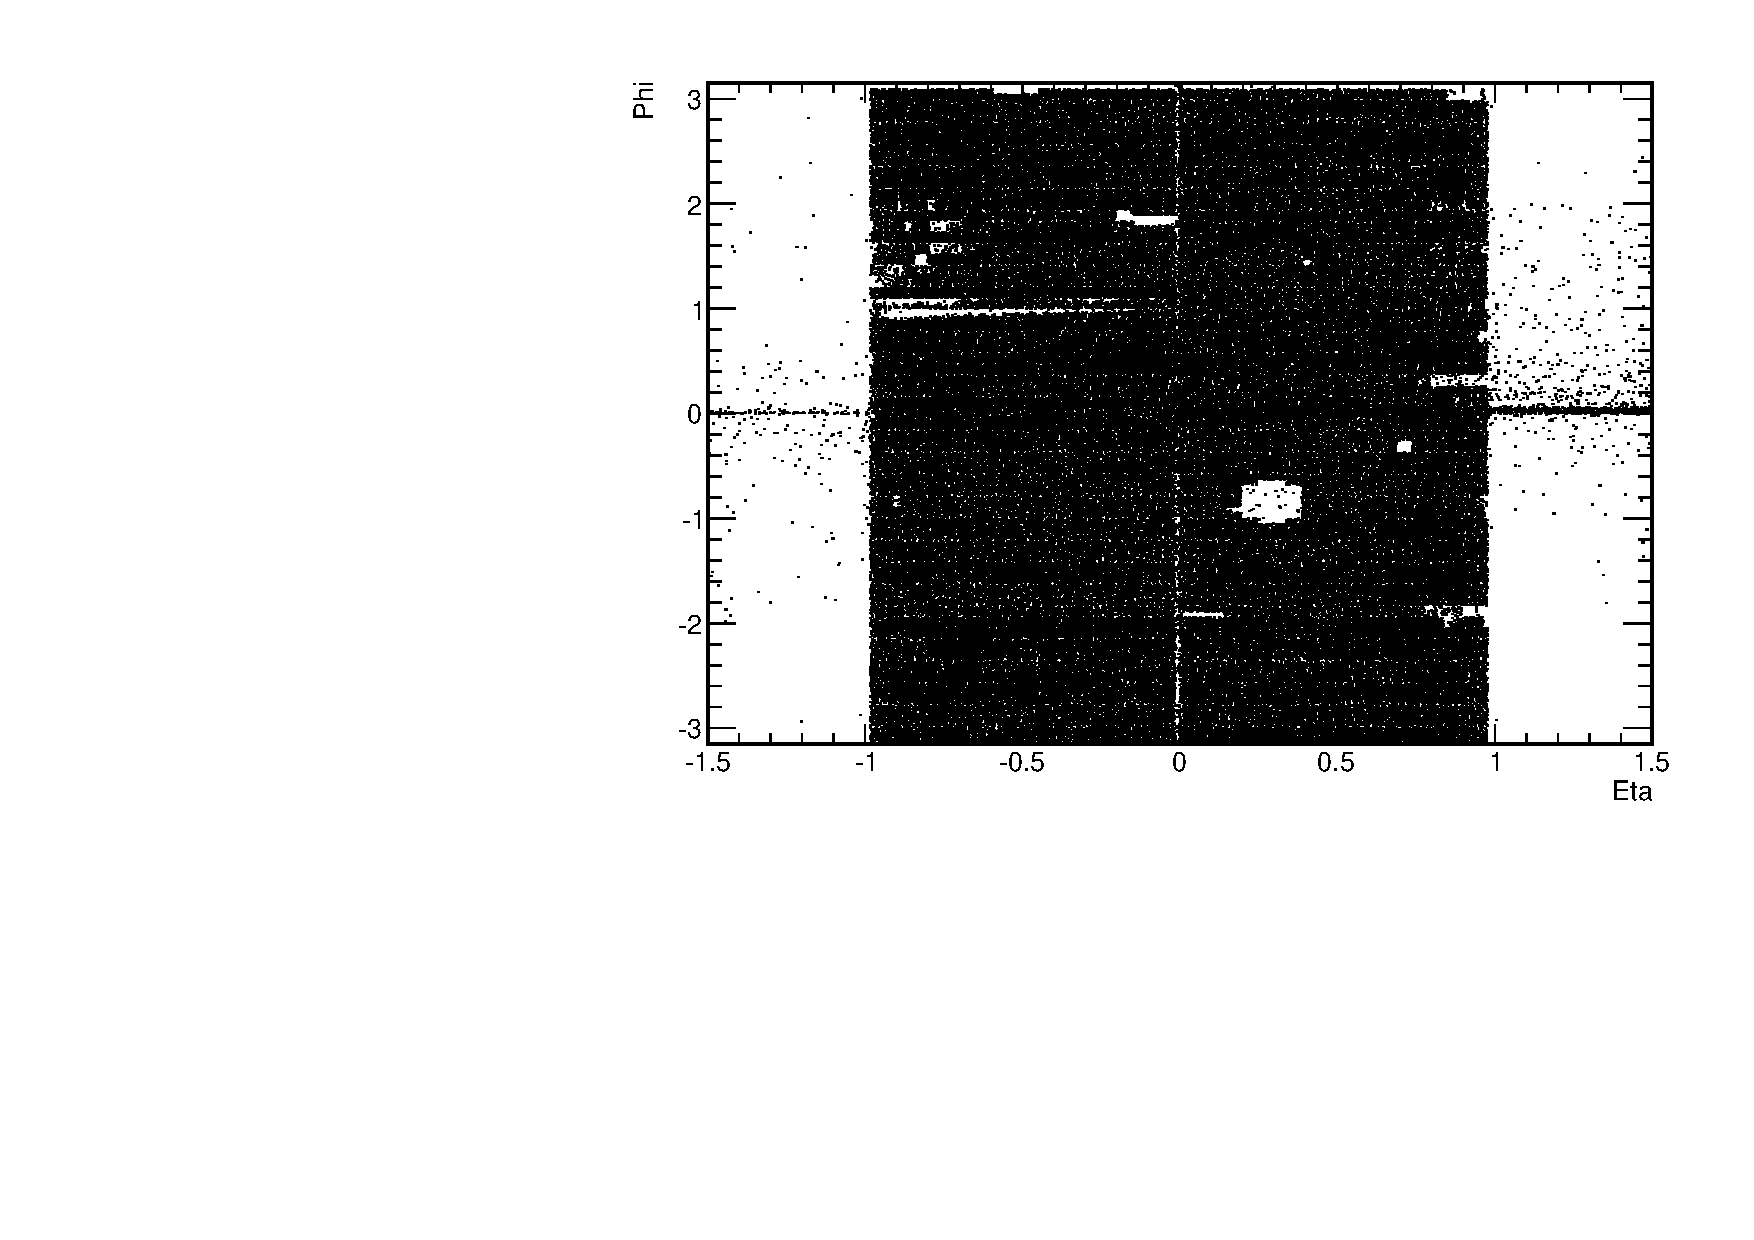
\includegraphics[scale=.8]{Plots/NPE/SMD_phi_eta.pdf}
\end{center}
\caption[SMD Point $\eta$ and $\phi$]{SMD points in $\eta$ and $\phi$ for the EMC points used in the analysis}
\label{fig:SMDetaphi}
\end{figure}

From the TPC we only consider tracks with $\pt$ above 1.5 GeV/c for association with points in the BEMC. When the TPC tracks are reconstructed they are fit to a helix to describe their trajectory through the TPC magnetic field. We then project these helices to the inner surface of the BEMC.

 

\section{Electron Identification}

\section{Electron Purity}

\section{Photonic Electron Identification}

\section{Photonic Electron Reconstruction Efficiency}
